% shared preamble of the theory figures (white background, purple / black theme, sans-serif)
\documentclass[tikz,border=8pt]{standalone}
\usepackage[T1]{fontenc}
\usepackage[scaled=0.92]{helvet}
\renewcommand{\familydefault}{\sfdefault}
\usepackage{amsmath,amssymb}
\usepackage[helvet]{sfmath}
\usetikzlibrary{arrows.meta,calc,decorations.pathreplacing,positioning,backgrounds}
\definecolor{ink}{HTML}{1A1A1F}
\definecolor{cohesin}{HTML}{6A3DE8}
\definecolor{condensin}{HTML}{1BAF7A}
\definecolor{fwd}{HTML}{D1303F}      % CTCF pointing right
\definecolor{rev}{HTML}{2B62D9}      % CTCF pointing left
\definecolor{panel}{HTML}{F8F6FD}
\definecolor{panelline}{HTML}{E3DDF5}
\tikzset{
  fiber/.style={line width=2.1pt,ink,line cap=round,line join=round},
  halo/.style={line width=6pt,white,line cap=round},
  lab/.style={font=\small,text=ink},
  note/.style={font=\footnotesize,text=ink!60},
  hd/.style={font=\bfseries\small,text=ink,anchor=west},
  leader/.style={line width=0.6pt,ink!45},
}
% soft panel, numbered badge, heading
\newcommand{\panelbg}[4]{\draw[rounded corners=9pt,fill=panel,draw=panelline,line width=0.9pt] (#1,#2) rectangle (#3,#4);}
\newcommand{\badge}[3]{\fill[ink] (#1,#2) circle (0.21);\node[white,font=\bfseries\footnotesize] at (#1,#2) {#3};}
% CTCF: a protein on the fibre carrying an arrow that gives the motif direction (f = right, r = left)
\newcommand{\protf}[2]{\draw[rounded corners=3.5pt,line width=0.6pt,draw=fwd!65!black,fill=fwd] (#1-0.3,#2-0.19) rectangle (#1+0.3,#2+0.19);
  \draw[white,line width=1.5pt,-{Stealth[length=3.4pt,width=4.4pt]}] (#1-0.15,#2)--(#1+0.16,#2);}
\newcommand{\protr}[2]{\draw[rounded corners=3.5pt,line width=0.6pt,draw=rev!65!black,fill=rev] (#1-0.3,#2-0.19) rectangle (#1+0.3,#2+0.19);
  \draw[white,line width=1.5pt,-{Stealth[length=3.4pt,width=4.4pt]}] (#1+0.15,#2)--(#1-0.16,#2);}
\newcommand{\prot}[3]{\csname prot#3\endcsname{#1}{#2}}
% ring seen at an angle, drawn as a tube (dark outline, light core); back half and front half
\newcommand{\ringpart}[5]{\draw[line width=4.6pt,#3!80!black,line cap=round] ([shift={(#1,#2)}]#4:0.55 and 0.21) arc[start angle=#4,end angle=#5,x radius=0.55,y radius=0.21];
  \draw[line width=2.4pt,#3!55!white,line cap=round] ([shift={(#1,#2)}]#4:0.55 and 0.21) arc[start angle=#4,end angle=#5,x radius=0.55,y radius=0.21];}
\newcommand{\ringback}[3]{\ringpart{#1}{#2}{#3}{180}{0}}
\newcommand{\ringfront}[3]{\ringpart{#1}{#2}{#3}{180}{360}}
% smooth loop whose foot (ring) is at (cx,y0): half-width W, height H, ring colour
\newcommand{\lloop}[5]{%
  \ringback{#1}{#2}{#5}%
  \draw[fiber] (#1-0.3,#2) .. controls (#1-0.3,#2+0.25*#4) and (#1-#3,#2+0.2*#4) .. (#1-#3,#2+0.55*#4)
     .. controls (#1-#3,#2+0.95*#4) and (#1-0.5*#3,#2+#4) .. (#1,#2+#4)
     .. controls (#1+0.5*#3,#2+#4) and (#1+#3,#2+0.95*#4) .. (#1+#3,#2+0.55*#4)
     .. controls (#1+#3,#2+0.2*#4) and (#1+0.3,#2+0.25*#4) .. (#1+0.3,#2);%
  \ringfront{#1}{#2}{#5}}
% gently undulating fibre from x0 to the loop foot at cx (height y0), and from x1
\newcommand{\base}[4]{%
  \draw[fiber] plot[smooth] coordinates {(#1,0.05) (#1+0.35*#3-0.35*#1,-0.05) (#3-1.4,0.04)} .. controls (#3-0.6,0.02) and (#3-0.3,0.05) .. (#3-0.3,#4);
  \draw[fiber] plot[smooth] coordinates {(#2,-0.05) (#2-0.35*#2+0.35*#3,0.05) (#3+1.4,-0.04)} .. controls (#3+0.6,-0.02) and (#3+0.3,0.05) .. (#3+0.3,#4);}
% stop sign for a blocked leg and a leg arrow
\newcommand{\stopbar}[3]{\draw[#3,line width=2.4pt,line cap=round] (#1,#2-0.2)--(#1,#2+0.2);}
\newcommand{\legarrow}[3]{\draw[cohesin,line width=1.6pt,-{Stealth[length=5pt,width=6pt]},line cap=round] (#1,#3)--(#2,#3);}

\tikzset{ln/.style={line width=0.7pt,ink!45},strand/.style={line width=2.4pt,ink,line cap=round},win/.style={rounded corners=2pt,draw=ink!50,dash pattern=on 2pt off 2pt,line width=0.8pt}}
\newcommand{\hitf}[3]{\draw[rounded corners=3.5pt,line width=0.6pt,draw=fwd!65!black,fill=fwd] (#1-0.9,#2-0.2) rectangle (#1+0.9,#2+0.2);\draw[white,line width=1.6pt,-{Stealth[length=3.6pt,width=4.6pt]}] (#1-0.6,#2)--(#1+0.6,#2);\node[note,anchor=south] at (#1,#2+0.25) {#3};}
\newcommand{\hitr}[3]{\draw[rounded corners=3.5pt,line width=0.6pt,draw=rev!65!black,fill=rev] (#1-0.9,#2-0.2) rectangle (#1+0.9,#2+0.2);\draw[white,line width=1.6pt,-{Stealth[length=3.6pt,width=4.6pt]}] (#1+0.6,#2)--(#1-0.6,#2);\node[note,anchor=north] at (#1,#2-0.25) {#3};}
\begin{document}
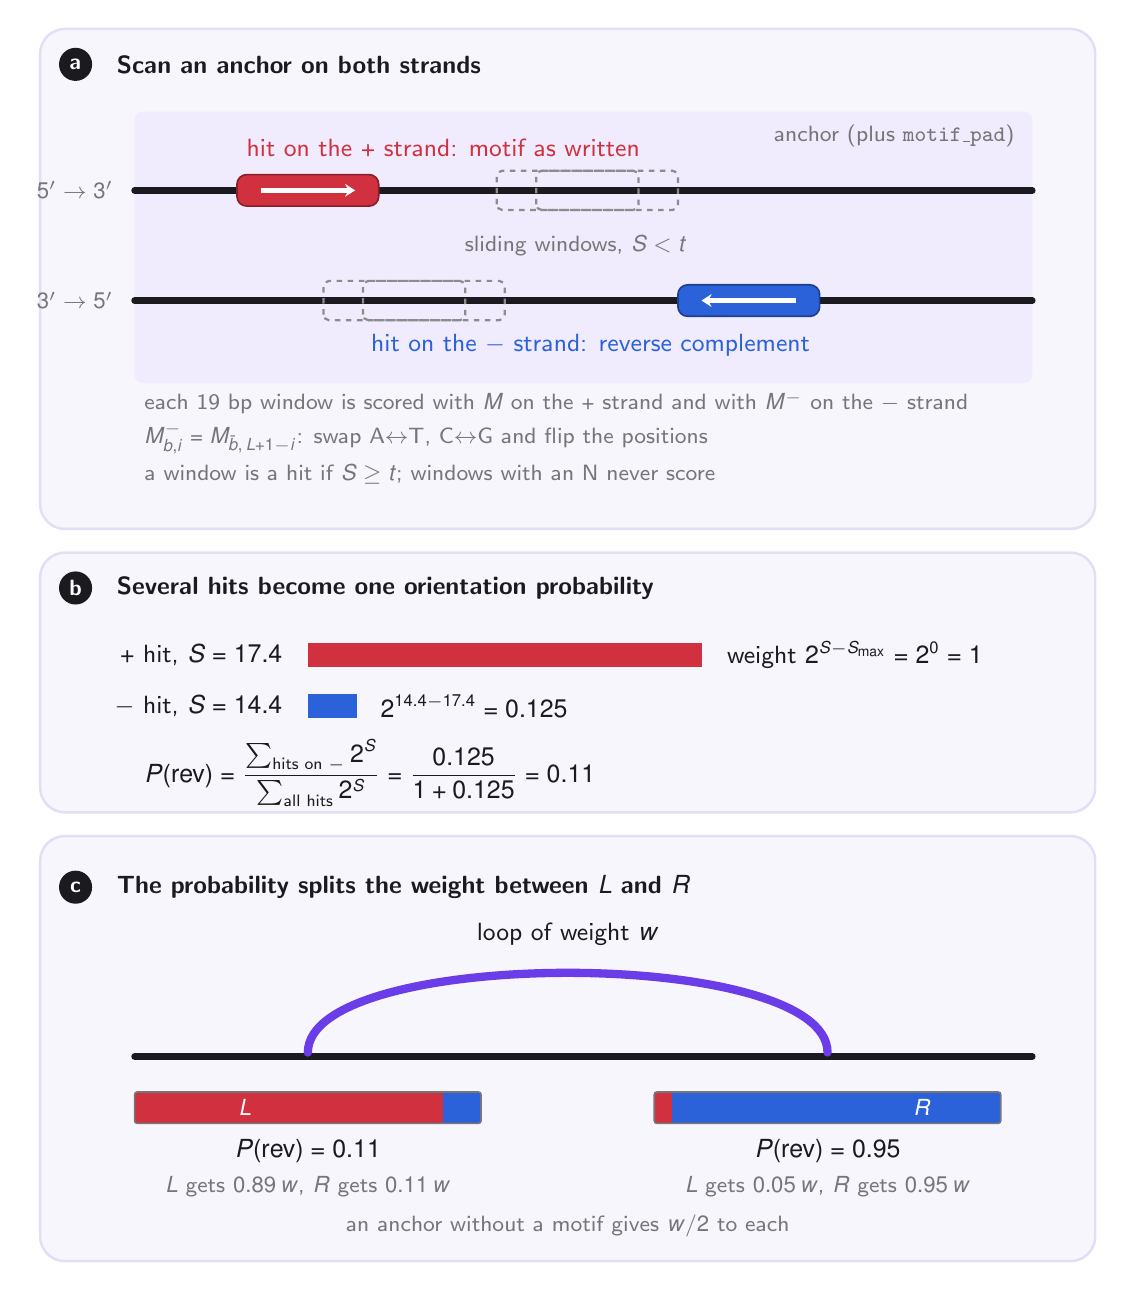
\begin{tikzpicture}
  \panelbg{0}{-3.6}{13.4}{2.75}\panelbg{0}{-7.2}{13.4}{-3.9}\panelbg{0}{-12.9}{13.4}{-7.5}
  % a: scan both strands
  \badge{0.45}{2.3}{a}\node[hd] at (0.85,2.3) {Scan an anchor on both strands};
  \fill[cohesin!10,rounded corners=3pt] (1.2,-1.75) rectangle (12.6,1.7);\node[note,anchor=north east] at (12.5,1.65) {anchor (plus \texttt{motif\_pad})};
  \draw[strand] (1.2,0.7)--(12.6,0.7);\draw[strand] (1.2,-0.7)--(12.6,-0.7);
  \node[note,anchor=east] at (1.05,0.7) {$5'\to3'$};\node[note,anchor=east] at (1.05,-0.7) {$3'\to5'$};
  \draw[win] (5.8,0.45) rectangle (7.6,0.95);\draw[win] (6.3,0.45) rectangle (8.1,0.95);\node[note] at (6.8,0.0) {sliding windows, $S<t$};
  \draw[win] (3.6,-0.95) rectangle (5.4,-0.45);\draw[win] (4.1,-0.95) rectangle (5.9,-0.45);
  \hitf{3.4}{0.7}{}\hitr{9.0}{-0.7}{}
  \node[lab,fwd,anchor=south west] at (2.5,1.0) {hit on the $+$ strand: motif as written};
  \node[lab,rev,anchor=north east] at (9.9,-1.0) {hit on the $-$ strand: reverse complement};
  \node[note,anchor=west] at (1.2,-2.0) {each 19 bp window is scored with $M$ on the $+$ strand and with $M^{-}$ on the $-$ strand};
  \node[note,anchor=west] at (1.2,-2.45) {$M^{-}_{b,i}=M_{\bar b,\,L+1-i}$: swap A$\leftrightarrow$T, C$\leftrightarrow$G and flip the positions};
  \node[note,anchor=west] at (1.2,-2.9) {a window is a hit if $S\ge t$; windows with an N never score};
  % b: hits to P(reverse)
  \badge{0.45}{-4.35}{b}\node[hd] at (0.85,-4.35) {Several hits become one orientation probability};
  \node[lab,anchor=east] at (3.2,-5.2) {$+$ hit, $S=17.4$};\node[lab,anchor=east] at (3.2,-5.85) {$-$ hit, $S=14.4$};
  \fill[fwd] (3.4,-5.35) rectangle (8.4,-5.05);\fill[rev] (3.4,-6.0) rectangle (3.4+0.625,-5.7);
  \node[lab,anchor=west] at (8.6,-5.2) {weight $2^{S-S_{\max}}=2^{0}=1$};\node[lab,anchor=west] at (4.2,-5.85) {$2^{14.4-17.4}=0.125$};
  \node[lab,anchor=west] at (1.2,-6.7) {$P(\mathrm{rev})=\dfrac{\sum_{\text{hits on }-}2^{S}}{\sum_{\text{all hits}}2^{S}}=\dfrac{0.125}{1+0.125}=0.11$};
  % c: probability to L and R
  \badge{0.45}{-8.15}{c}\node[hd] at (0.85,-8.15) {The probability splits the weight between $L$ and $R$};
  \draw[strand] (1.2,-10.3)--(12.6,-10.3);
  \draw[cohesin,line width=3pt,line cap=round] (3.4,-10.25) .. controls (3.4,-8.9) and (10.0,-8.9) .. (10.0,-10.25);
  \node[lab] at (6.7,-8.75) {loop of weight $w$};
  \legdot{3.4}{-10.3}{cohesin}\legdot{10.0}{-10.3}{cohesin}
  % each anchor: its weight split into an L share (red) and an R share (blue)
  \foreach \x/\pr in {3.4/0.11,10.0/0.95}{
    \pgfmathsetmacro{\wl}{(1-\pr)*4.4}\pgfmathsetmacro{\xm}{\x-2.2+\wl}\pgfmathsetmacro{\xr}{\x+2.2}\pgfmathsetmacro{\xl}{\x-2.2}
    \fill[fwd] (\xl,-10.75) rectangle (\xm,-11.15);\fill[rev] (\xm,-10.75) rectangle (\xr,-11.15);
    \draw[ink!60,line width=0.6pt,rounded corners=1pt] (\xl,-10.75) rectangle (\xr,-11.15);}
  \node[white,font=\footnotesize\bfseries] at (2.6,-10.95) {$L$};\node[white,font=\footnotesize\bfseries] at (11.2,-10.95) {$R$};
  \node[lab] at (3.4,-11.5) {$P(\mathrm{rev})=0.11$};\node[lab] at (10.0,-11.5) {$P(\mathrm{rev})=0.95$};
  \node[note] at (3.4,-11.95) {$L$ gets $0.89\,w$, $R$ gets $0.11\,w$};\node[note] at (10.0,-11.95) {$L$ gets $0.05\,w$, $R$ gets $0.95\,w$};
  \node[note] at (6.7,-12.45) {an anchor without a motif gives $w/2$ to each};
\end{tikzpicture}
\end{document}
